%Version 2.1 April 2023
% See section 11 of the User Manual for version history
%
%%%%%%%%%%%%%%%%%%%%%%%%%%%%%%%%%%%%%%%%%%%%%%%%%%%%%%%%%%%%%%%%%%%%%%
%%                                                                 %%
%% Please do not use \input{...} to include other tex files.       %%
%% Submit your LaTeX manuscript as one .tex document.              %%
%%                                                                 %%
%% All additional figures and files should be attached             %%
%% separately and not embedded in the \TeX\ document itself.       %%
%%                                                                 %%
%%%%%%%%%%%%%%%%%%%%%%%%%%%%%%%%%%%%%%%%%%%%%%%%%%%%%%%%%%%%%%%%%%%%%

%%\documentclass[referee,sn-basic]{sn-jnl}% referee option is meant for double line spacing

%%=======================================================%%
%% to print line numbers in the margin use lineno option %%
%%=======================================================%%

%%\documentclass[lineno,sn-basic]{sn-jnl}% Basic Springer Nature Reference Style/Chemistry Reference Style

%%======================================================%%
%% to compile with pdflatex/xelatex use pdflatex option %%
%%======================================================%%

%%\documentclass[pdflatex,sn-basic]{sn-jnl}% Basic Springer Nature Reference Style/Chemistry Reference Style


%%Note: the following reference styles support Namedate and Numbered referencing. By default the style follows the most common style. To switch between the options you can add or remove “Numbered” in the optional parenthesis. 
%%The option is available for: sn-basic.bst, sn-vancouver.bst, sn-chicago.bst, sn-mathphys.bst. %  
 
%%\documentclass[sn-nature]{sn-jnl}% Style for submissions to Nature Portfolio journals
%%\documentclass[sn-basic]{sn-jnl}% Basic Springer Nature Reference Style/Chemistry Reference Style
\documentclass[sn-mathphys,Numbered]{sn-jnl}% Math and Physical Sciences Reference Style
%%\documentclass[sn-aps]{sn-jnl}% American Physical Society (APS) Reference Style
%%\documentclass[sn-vancouver,Numbered]{sn-jnl}% Vancouver Reference Style
%%\documentclass[sn-apa]{sn-jnl}% APA Reference Style 
%%\documentclass[sn-chicago]{sn-jnl}% Chicago-based Humanities Reference Style
%%\documentclass[default]{sn-jnl}% Default
%%\documentclass[default,iicol]{sn-jnl}% Default with double column layout

%%%% Standard Packages
%%<additional latex packages if required can be included here>

\usepackage{graphicx}%
\usepackage{multirow}%
\usepackage{amsmath,amssymb,amsfonts}%
\usepackage{amsthm}%
\usepackage{mathrsfs}%
\usepackage[title]{appendix}%
\usepackage{xcolor}%
\usepackage{textcomp}%
\usepackage{manyfoot}%
\usepackage{booktabs}%
% \usepackage{algorithm}%
\usepackage{algorithmicx}%
\usepackage{algpseudocode}%
\usepackage{listings}%

\usepackage{float}
\usepackage{amsmath}
\usepackage[ruled,linesnumbered]{algorithm2e}

%%%%

%%%%%=============================================================================%%%%
%%%%  Remarks: This template is provided to aid authors with the preparation
%%%%  of original research articles intended for submission to journals published 
%%%%  by Springer Nature. The guidance has been prepared in partnership with 
%%%%  production teams to conform to Springer Nature technical requirements. 
%%%%  Editorial and presentation requirements differ among journal portfolios and 
%%%%  research disciplines. You may find sections in this template are irrelevant 
%%%%  to your work and are empowered to omit any such section if allowed by the 
%%%%  journal you intend to submit to. The submission guidelines and policies 
%%%%  of the journal take precedence. A detailed User Manual is available in the 
%%%%  template package for technical guidance.
%%%%%=============================================================================%%%%

%\jyear{2021}%

%% as per the requirement new theorem styles can be included as shown below
\theoremstyle{thmstyleone}%
\newtheorem{theorem}{Theorem}%  meant for continuous numbers
%%\newtheorem{theorem}{Theorem}[section]% meant for sectionwise numbers
%% optional argument [theorem] produces theorem numbering sequence instead of independent numbers for Proposition
\newtheorem{proposition}[theorem]{Proposition}% 
%%\newtheorem{proposition}{Proposition}% to get separate numbers for theorem and proposition etc.

\theoremstyle{thmstyletwo}%
\newtheorem{example}{Example}%
\newtheorem{remark}{Remark}%

\theoremstyle{thmstylethree}%
\newtheorem{definition}{Definition}%

\raggedbottom
%%\unnumbered% uncomment this for unnumbered level heads

\begin{document}

\title[ASISO: A Robust and Stable Data Synthesis Method to Optimize Samples ]{ASISO: A Robust and Stable Data Synthesis Method to Optimize Samples }

%%=============================================================%%
%% Prefix	-> \pfx{Dr}
%% GivenName	-> \fnm{Joergen W.}
%% Particle	-> \spfx{van der} -> surname prefix
%% FamilyName	-> \sur{Ploeg}
%% Suffix	-> \sfx{IV}
%% NatureName	-> \tanm{Poet Laureate} -> Title after name
%% Degrees	-> \dgr{MSc, PhD}
%% \author*[1,2]{\pfx{Dr} \fnm{Joergen W.} \spfx{van der} \sur{Ploeg} \sfx{IV} \tanm{Poet Laureate} 
%%                 \dgr{MSc, PhD}}\email{iauthor@gmail.com}
%%=============================================================%%

\author[1]{\fnm{Yukun} \sur{Du}}\email{mg2108129@stu.nau.edu.cn}

\author[2]{\fnm{Yitao} \sur{Cai}}\email{ma2208133@stu.nau.edu.cn}

\author*[3]{\fnm{Ming} \sur{Lu}}\email{lumin@nau.edu.cn}

\author[4]{\fnm{Yao} \sur{Li}}\email{223080612@stu.nau.edu.cn}


\affil*[1]{\orgdiv{School of Statistics and Data Science}, \orgname{Nanjing Audit University}, \orgaddress{\city{Nanjing}, \postcode{211815}, \country{China}}}

\affil*[2]{\orgdiv{School of Statistics and Data Science}, \orgname{Nanjing Audit University}, \orgaddress{\city{Nanjing}, \postcode{211815}, \country{China}}}

\affil*[3]{\orgdiv{School of Statistics and Data Science}, \orgname{Nanjing Audit University}, \orgaddress{\city{Nanjing}, \postcode{211815}, \country{China}}}

\affil*[4]{\orgdiv{School of Statistics and Data Science}, \orgname{Nanjing Audit University}, \orgaddress{\city{Nanjing}, \postcode{211815}, \country{China}}}


%%==================================%%
%% sample for unstructured abstract %%
%%==================================%%

\abstract{Most existing data synthesis methods are designed to tackle problems such as dataset imbalance, data anonymization and insufficient sample size. There is a lack of effective synthesis methods for the limited number of datasets which contain a large of features and unknown noise to expand the size of the dataset. We propose a data synthesis method, named Adaptive Subspace Interpolation for Sample Optimization (ASISO). The idea is to divide the original feature space into several subspaces with an equal number of samples, and then perform interpolation for the samples in the adjacent subspaces. This method can adaptively adjust the size of the dataset containing unknown noise, and the expanded data typically contain minimal error with actual. Moreover, it adjusts the structure of the samples, which can significantly reduce the proportion of samples with large errors. In addition, the hyperparameters of this method have an intuitive explanation and usually require little calibration. Experimental results on artificial data and benchmark data sets demonstrate that ASISO is a robust and stable method to optimize samples.}
\keywords{Data synthesis, Unknown noise, Interpolation, Sample optimization, Robust}


%%================================%%
%% Sample for structured abstract %%
%%================================%%

% \abstract{\textbf{Purpose:} The abstract serves both as a general introduction to the topic and as a brief, non-technical summary of the main results and their implications. The abstract must not include subheadings (unless expressly permitted in the journal's Instructions to Authors), equations or citations. As a guide the abstract should not exceed 200 words. Most journals do not set a hard limit however authors are advised to check the author instructions for the journal they are submitting to.
% 
% \textbf{Methods:} The abstract serves both as a general introduction to the topic and as a brief, non-technical summary of the main results and their implications. The abstract must not include subheadings (unless expressly permitted in the journal's Instructions to Authors), equations or citations. As a guide the abstract should not exceed 200 words. Most journals do not set a hard limit however authors are advised to check the author instructions for the journal they are submitting to.
% 
% \textbf{Results:} The abstract serves both as a general introduction to the topic and as a brief, non-technical summary of the main results and their implications. The abstract must not include subheadings (unless expressly permitted in the journal's Instructions to Authors), equations or citations. As a guide the abstract should not exceed 200 words. Most journals do not set a hard limit however authors are advised to check the author instructions for the journal they are submitting to.
% 
% \textbf{Conclusion:} The abstract serves both as a general introduction to the topic and as a brief, non-technical summary of the main results and their implications. The abstract must not include subheadings (unless expressly permitted in the journal's Instructions to Authors), equations or citations. As a guide the abstract should not exceed 200 words. Most journals do not set a hard limit however authors are advised to check the author instructions for the journal they are submitting to.}

\keywords{Data synthesis, Unknown noise, Interpolation, Sample optimization, Robust}

%%\pacs[JEL Classification]{D8, H51}

%%\pacs[MSC Classification]{35A01, 65L10, 65L12, 65L20, 65L70}

\maketitle

\section{Introduction}\label{sec1}

Synthetic data presents an effective solution to the challenges of inadequate or low-quality sample, particularly in the era of big data. Through the use of data synthesis methods to generate synthetic data, it provides a cost-effective and efficient alternative to collecting and labeling large amounts of real-world data. Furthermore, these methods can address privacy concerns associated with real-world data, making it safer to share and analyze \cite{bib1}. Recently, there has been a surge in the use of synthetic data in machine learning, with various synthetic methods being developed \cite{bib2,bib3}.

Representative data synthesis methods can be classified into three categories. The first category entails techniques such as interpolation, extrapolation, and other methods \cite{bib4} that generate additional data points representative of the underlying distribution. These methods improve the quality of the dataset and model generalization. For image data, deep learning-based methods such as VAE and GAN can also be used to generate new data \cite{bib5,bib6}. These methods are useful for improving the quality of the dataset and model generalization. The second category is to address the issue of dataset imbalance, such as SMOTE \cite{bib7}, and some of its enhancements \cite{bib8,bib9,bib10}. These methods can synthesize minority class samples to balance the dataset and improve the model's performance. Finally, data sharing and research require sensitive data privacy protection. Synthetic data can help protect sensitive information while still enabling data sharing and research. Normally, we can add random noise to protect original data, generating synthetic data for sharing and research purposes like differential privacy methods \cite{bib11}. Overall, these methods help optimize the representation and use of data in various applications.

For some actual tasks, original data often contains a multitude of features and unknown noise \cite{bib12}. Since synthetic method involves generating new data based on existing data, the quality of the new points depends on the quality and quantity of the original data. If the quality of the original data is poor or the quantity is insufficient, then the synthetic data may have limitations in terms of its quality \cite{bib13}. However, there exists a lack of effective synthetic methods for datasets with a restricted size and complex noise to expand the size of data set.

Based on the purpose of improving the quality and quantity of the dataset, and motivated by piecewise linear interpolation and spline interpolation, we propose a robust and stable data synthesis method named Adaptive Subspace Interpolation for Sample Optimization (ASISO), which aims to adaptively adjust the sample size and structure of the original dataset containing unknown noise. The idea is to divide the original feature space into several subspaces with an equal number of samples, and then perform linear interpolation for the samples in the adjacent subspaces. This method achieves sample optimization in two aspects. First, it can adaptively adjust the size of the dataset, and the expanded data typically contains minimal error with actual. Second, it adjusts the structure of the samples, which can significantly reduce the proportion of samples with large errors, thereby minimizing the impact of noise for model generalization.

The rest of this paper is organized as follows. Section 2 reviews the research of existing interpolation. Section 3 details the concept of the proposed ASISO method and provides proof for the effectiveness of this method. Experimental results are presented and analyzed in Section 4. Finally, we conclude this paper in Section 5.

\section{Related Work}\label{sec2}

Traditional interpolation methods are based on the function values of known data points for extrapolation and prediction. For a given data set, there are generally two cases. In the case of two known data points and interpolation in between, interpolation can be selected based on distance, such as nearest-neighbor interpolation \cite{bib14}. If it is assumed that the unknown point between these two data points is consistent with the straight line between them, a linear function can be used to fit and interpolate, such as linear interpolation, piecewise linear interpolation \cite{bib15,bib16}. For interpolation among multiple given points, a commonly used method is to predict the value of the unknown point by constructing a high-degree polynomial based on the given points, such as Lagrange interpolation, Newton interpolation \cite{bib17,bib18}. However, with an increase in the number of data points and the degree of the polynomial, there is a risk of overfitting and numerical instability (Runge's phenomenon) \cite{bib19}. Another solution is to construct a global smooth function by fitting a low-degree polynomial in a local region. In comparison to high-degree polynomial interpolation methods, this method has better smoothness and numerical stability, such as spline interpolation \cite{bib20}. Nevertheless, as it is necessary to fit multiple local low-degree polynomials, this method can lead to relatively high computational complexity.

When expanding the sample size using interpolation methods, the selection of node positions and quantities has a significant impact on the accuracy and stability of interpolation results. Typically, equidistant nodes \cite{bib21} are used for interpolation position selection, where nodes are equally spaced within the interpolation interval. Chebyshev nodes \cite{bib22} are selected within the interpolation interval to satisfy certain conditions for better fitting of the function. In addition, the choice of the number of interpolations can lead to instability of the data and insufficient validation accuracy. One way to determine the appropriate number of interpolations is by comparing the fitting degree of the model trained under different interpolation numbers with the original data, but this may lead to overfitting and poor generalization ability of the model.

\section{Proposed Method}\label{sec3}

In this section, we will explain the proposed ASISO method in detail. ASISO introduces two algorithms: K-Space and K-Match. To clearly illustrate the proposed method, we will first provide an overview of ASISO and then introduce the specific algorithms involved. 

\subsection{Overview}\label{subsec1}

The ASISO is mainly based on the linear interpolation to increase the size and improve the quality of the original dataset. The idea is to divide the original feature space into several subspaces with an equal number of samples, and then perform linear interpolation for the samples in the adjacent subspaces. This method requires two hyperparameters ($k$ and $\eta$) in advance. Interpretation of parameter $k$ is the number of samples existing in each feature subspace, while $\eta$ is the number of equidistant nodes interpolated per unit distance in the linear interpolation of the samples. This proposed method is illustrated in Figure~\ref{fig1}.

\begin{figure}[H]%
\centering
\vspace{-1.6cm}   %调整图片与上文的垂直距离 
\setlength{\abovecaptionskip}{0.cm} %调整标题上方的距离 
\setlength{\abovecaptionskip}{-1.5cm} %调整标题下方的距离
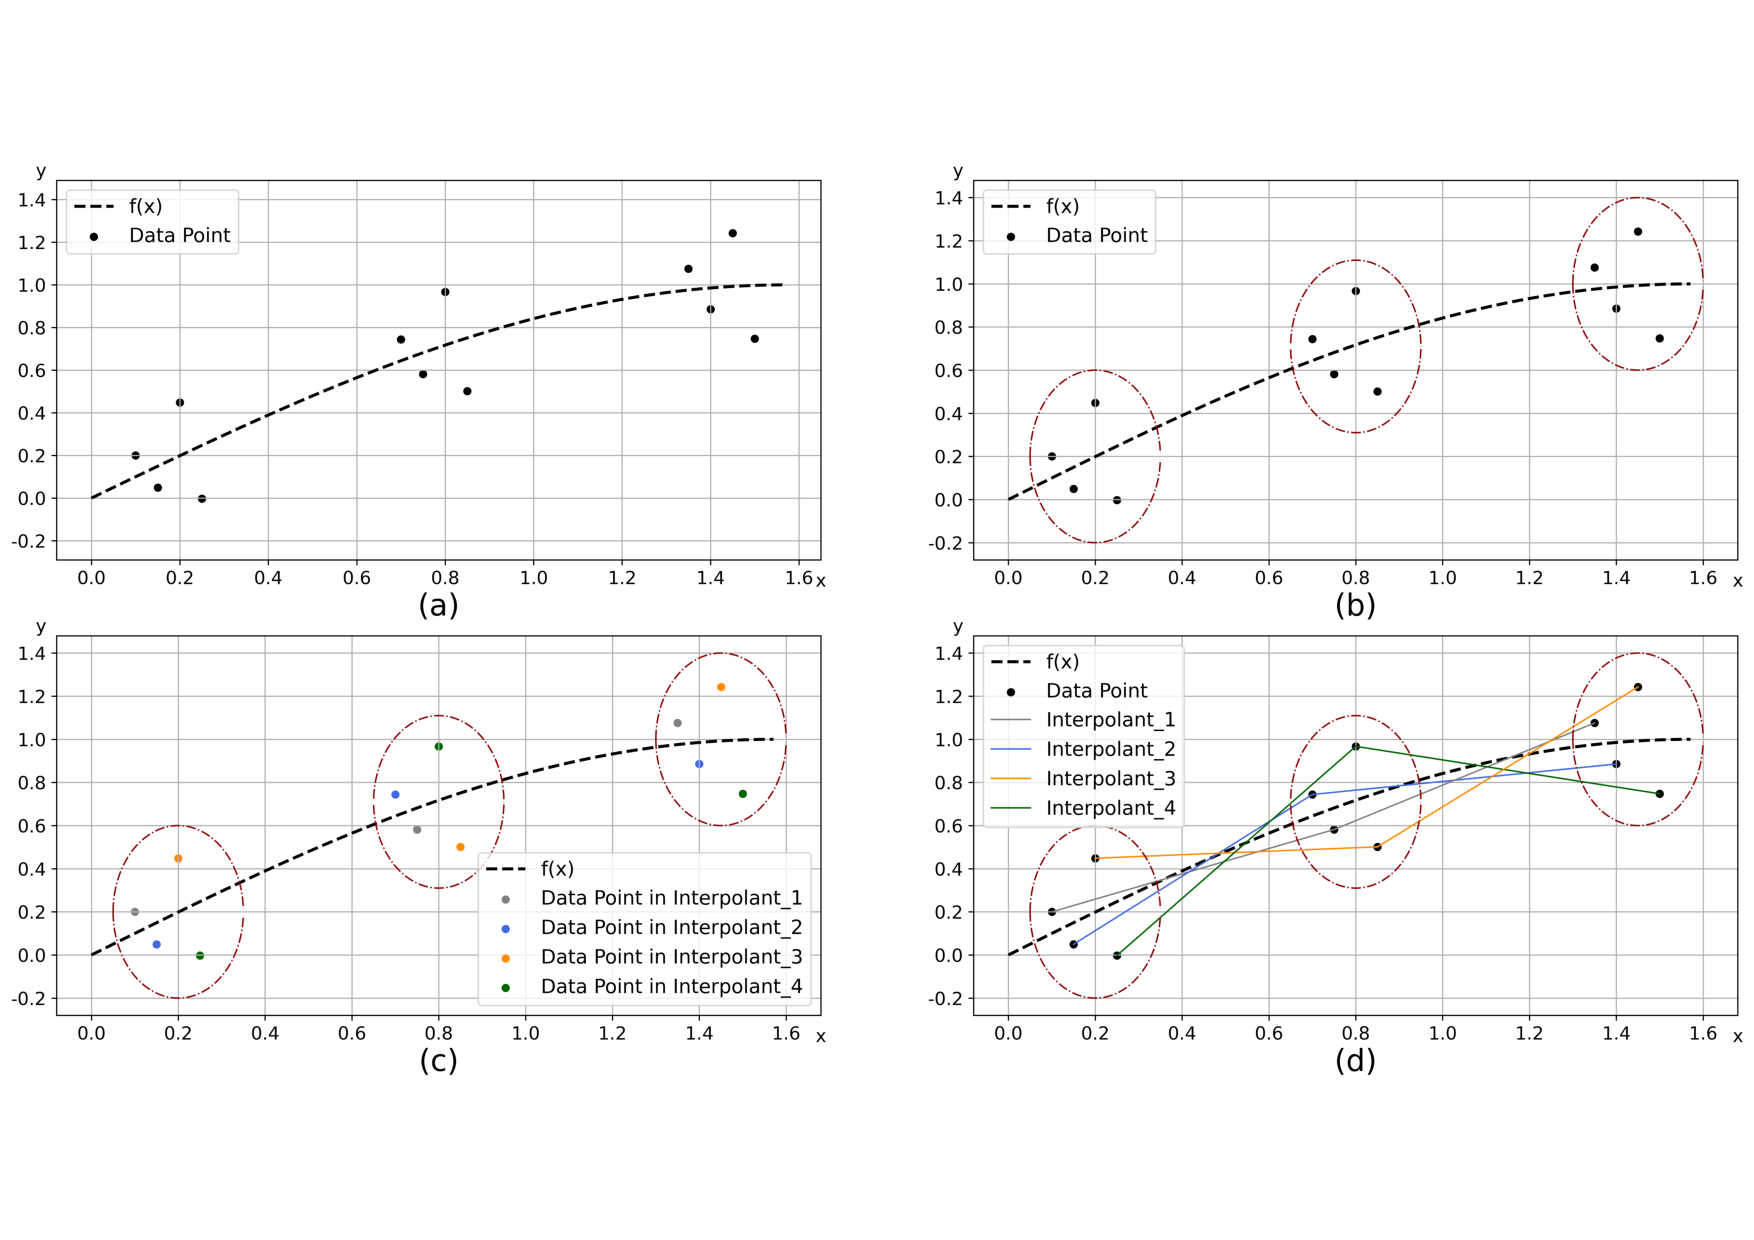
\includegraphics[width=1\textwidth]{fig1.pdf}
\caption{Overview of the proposed approach for ASISO. (a) The dataset contains multiple noisy samples, and the true functional relationship between $x$ and $y$ is $f(\cdot)$. (b) In the first step, we use the K-Space algorithm to perform unsupervised clustering on the dataset and divide the original feature space into several subspaces. (c) Interpolation matching of samples between adjacent subspaces is performed using the K-Match algorithm, and sample points with the same color belong to the same class to be interpolated. (d) Piecewise linear interpolation is performed on samples under different classes, and inserting equidistant sample points on lines of different colors in adjacent subspaces.}\label{fig1}
\end{figure}

The data set $D=\{\boldsymbol{x}_i,y_i\}_{i=1}^n$ has been given and is assumed to be contaminated with unknown noise, where $\boldsymbol{x}_i\in\mathcal{X}=R^p$ and $y_i\in\mathcal{Y}=R$. Assuming $\dot{y}_i=f(\dot{\boldsymbol{x}}_i)$ where $\dot{\boldsymbol{x}}_i$ is the actual value of $\boldsymbol{x}_i$, $\dot{y}_i$ is the actual value of $y_i$ and $f(\cdot)$ is a continuous function, represents the relationship in reality between $\boldsymbol{x}_i$ and $y$. Consider the model:

\begin{equation}
\dot{y}_i+\epsilon_{i,y}=f(\dot{\boldsymbol{x}}_i+\boldsymbol{\epsilon}_{i,x})+\epsilon_i,\label{eq1}
\end{equation}
where $\epsilon_{i,y}$ is the noise in $\dot{y}_i$, $\boldsymbol{\epsilon}_{i,x}$ is the noise in $\dot{\boldsymbol{x}}_i$, and $\epsilon_i$ represents the error term. The expression \eqref{eq1} can be rewritten as:

\begin{equation}
y_i=f(\boldsymbol{x}_i)+\epsilon_i.\label{eq2}
\end{equation}
Let $\boldsymbol{x}_0=\{x_0^1,\ldots,x_0^p\}$, we have $x_0^j=inf\{x_i^j\}_{i=1}^n$ for $\forall j=1,\ldots,p$, and call $\boldsymbol{x}_0$ the sample minimum point. 

Given the hyperparameter $k$, we provide an unsupervised clustering method called K-Space. As it is shown in Figure~\ref{fig1}(b), the space can be partitioned into $n/k$ subspaces, each containing $k$ samples. i.e., $\mathcal{X}=\cup_{s=1}^{n/k}\mathcal{X}_s$, $\mathcal{X}_i\cap\mathcal{X}_j=\emptyset,i,j=1,2,\ldots,\frac{n}{k}$ and $i\neq j$ the datasets corresponding to different subspaces $\mathcal{D}=\cup_{s=1}^{n/k}\mathcal{D}_s,\mathcal{D}_s=\{(\boldsymbol{x}_i^s,y_i^s)\}_{i=1}^k$, $\boldsymbol{x}_i^s\in\mathcal{X}_s$. For two adjacent subspaces, since $f(\cdot)$ is a continuous function, we assume that it can be approximated as a linear function $g(\cdot)$, and then \eqref{eq2} can be transformed into:

\begin{equation}
y_i=g(\boldsymbol{x}_i)+\epsilon_i+\epsilon_i^\prime,\label{eq3}
\end{equation}
where $\epsilon_i^\prime$ is the linear fitting error term. When the distance between two adjacent subspaces approaches zero and the measurements of subspaces tend to zero, obtain $\epsilon_i^\prime\rightarrow0$. Next, we will perform sample interpolation between adjacent subspaces.

We need to calculate the centers of each cluster, as follow:

\begin{equation}
\overline{\boldsymbol{x}}^s=\dfrac{1}{k}\sum\limits_{\boldsymbol{x}_i^s\in\mathcal{D}_s}\boldsymbol{x}_i^s.\label{eq4}
\end{equation}
To make $\epsilon_i^\prime\rightarrow0$, we need to ensure that the interpolation is performed between clusters that are close in distance as much as possible. Among $\{\mathcal{D}_s\}_{s=1}^{n/k}$, we define $\mathcal{D}_{(1)}$ whose cluster center has the minimum distance to the sample minimum point $\boldsymbol{x}_0$, and define $\mathcal{D}_{(d)}$ whose cluster center has the minimum distance to the center of $\mathcal{D}_{(d-1)},\mathcal{D}_{(d-1)}\neq\mathcal{D}_{(1)},\ldots,\mathcal{D}_{(d-1)}$ and $d>1$.

\begin{equation}
D_{(1)}=\mathop{argmin}\limits_{\mathcal{D}_s\in\mathcal{D}}dist(\boldsymbol{x}_0,\overline{\boldsymbol{x}}^s),\label{eq5}
\end{equation}

\begin{equation}
D_{(d)}=\mathop{argmin}\limits_{\{\mathcal{D}_s\in\mathcal{D}\},\mathcal{D}_s\neq\mathcal{D}_{(1)},\ldots,\mathcal{D}_{(d-1)}}dist(\overline{\boldsymbol{x}}_0^{(d-1)},\overline{\boldsymbol{x}}^s),\label{eq6}
\end{equation}
where $\overline{\boldsymbol{x}}^{(d-1)}$ is the center of $\mathcal{D}_{(d-1)}$. Perform interpolation in $\{\mathcal{D}_{(d)}\}_{d=1}^{n/k}$ sequentially according to the order of $d$ values, and interpolate only between adjacent subspaces (i.e., interpolate between $\mathcal{D}_{(1)}$ and $\mathcal{D}_{(2)}$, between $\mathcal{D}_{(2)}$ and $\mathcal{D}_{(3)}$, and so on). 

When performing linear interpolation between adjacent subspaces, we should pair the $k$ samples from the first subspace with an equal number of samples from the second subspace. The interpolation rules between adjacent subspaces are as follows:

\begin{enumerate}[2.]

\item Linear interpolation can only be performed between two samples belonging to different adjacent subspace sets.

\item Interpolation must be performed for each sample.

\item Participation of each sample point is restricted to a single interpolation instance. 

\end{enumerate}

The number of matching schemes is $k!$. As it is shown in Figure~\ref{fig1}(c), we provide a matching method called K-Match. Suppose $\epsilon_i^\prime\rightarrow0$, this method can select a good-performing matching scheme $\{(\boldsymbol{x}_i^{(d)},y_i^{(d)}),(\boldsymbol{x}_i^{(d+1)},y_i^{(d+1)})\}_{i=1}^k$ from $k!$.

Assuming $\boldsymbol{x}$ and $y$ are continuous variables. Given another hyperparameter $\eta$, the number of samples inserted using linear interpolation method between $\mathcal{D}_{(d)}$ and $\mathcal{D}_{(d+1)}$ is $\sum\limits_{i=1}^k\lfloor\eta\cdot dist(\boldsymbol{x}_i^{(d)},\boldsymbol{x}_i^{(d+1)})\rfloor$. Taking $(\boldsymbol{x}_i^{(d)},y_i^{(d)})\in\mathcal{D}_{(d)}$ and $(\boldsymbol{x}_i^{(d+1)},y_i^{(d+1)})\in\mathcal{D}_{(d+1)}$ as example, $\{(\boldsymbol{x}_{(d,d+1)}^{(m,i)},y_{(d,d+1)}^{(m,i)})\}_{m=1}^{\lfloor\eta\cdot dist(\boldsymbol{x}_i^{(d)},\boldsymbol{x}_i^{(d+1)})\rfloor}$ is the set of inserted samples, the linear interpolation formula is defined as:

\begin{equation}
\boldsymbol{x}_{(d,d+1)}^{(m,i)}=\boldsymbol{x}_i^{(d)}+m\cdot\dfrac{\boldsymbol{x}_i^{(d+1)}-\boldsymbol{x}_i^{(d)}}{\lfloor\eta\cdot dist(\boldsymbol{x}_i^{(d)},\boldsymbol{x}_i^{(d+1)})\rfloor+1},\label{eq7}
\end{equation}

\begin{equation}
y_{(d,d+1)}^{(m,i)}=y_i^{(d)}+m\cdot\dfrac{y_i^{(d+1)}-y_i^{(d)}}{\lfloor\eta\cdot dist(y_i^{(d)},y_i^{(d+1)})\rfloor+1}.\label{eq8}
\end{equation}
After ASISO processing, the original dataset will be optimized. The main steps of the ASISO algorithm are summarized in Algorithm~\ref{algo1}.

\begin{algorithm}[H] 
	\caption{ASISO}
	\label{algo1}
	\KwIn{Data set $D=\{(\boldsymbol{x}_i,y_i\}_{i=1}^n$; hyperparameters $k$ and $\eta$}
	\KwOut{Optimized data set $D^\prime$}  
	\BlankLine
	Perform unsupervised clustering using K-Space obtain: 
        $D=\{D_s\}_{s=1}^{n/k}$, where $D_s=\{\boldsymbol{x}_i^s,y_i^s\}_{i=1}^k$

        Calculate culster centers of each cluster: 
        $\{\overline{\boldsymbol{x}}^s\}_{s=1}^{n/k}$

        Obtain $\{D_{(d)}\}_{d=1^{n/k}}$ based on \eqref{eq5} and \eqref{eq6}
        
	\For{\textnormal{$d=1,\ldots,\frac{n}{k}-1$}}{
		Matching samples between $D_{(d)}$ and $D_{(d+1)}$ using K-Match obtain 
        $\{(\boldsymbol{x}_i^{(d)},y_i^{(d)}),(\boldsymbol{x}_i^{(d+1)},y_i^{(d+1)})\}$
		
		\For{$i=1,\ldots,k$}{
			Synthesize new samples 
   $\{(\boldsymbol{x}_{(d,d+1)}^{(m,i)},y_{(d,d+1)}^{(m,i)})\}_{m=1}^{\lfloor\eta\cdot dist(\boldsymbol{x}_i^{(d)},\boldsymbol{x}_i^{(d+1)})\rfloor}$ 
                using \eqref{eq7} and \eqref{eq8}

                $D^\prime\leftarrow\{(\boldsymbol{x}_{(d,d+1)}^{(m,i)},y_{(d,d+1)}^{(m,i)})\}_{m=1}^{\lfloor\eta\cdot dist(\boldsymbol{x}_i^{(d)},\boldsymbol{x}_i^{(d+1)})\rfloor}$
	}
    }
\end{algorithm}

The assumptions of ASISO are as follows:

\begin{enumerate}[2.]

\item $f(\cdot)$ is a continuous function.

\item the linear fitting error $\epsilon_i^\prime\rightarrow0$.

\item $\boldsymbol{x}$ and $y$ are continuous variables.

\end{enumerate}


\subsection{K-Space}\label{subsec2}

The implementation of ASISO requires an unsupervised clustering method to partition the feature space into multiple subspaces, each containing $k$ samples. Based on this, we propose the K-Space clustering method. The clustering method has the following performance:

\begin{enumerate}[1.]

\item Each subspace contains an equal number of samples, i.e., $\mathcal{D}=\cup_{s=1}^{n/k}\mathcal{D}_s,\mathcal{D}_s=\{(\boldsymbol{x}_i^s,y_i^s)\}_{{i=1}}^k$;

\item Each sample belongs to only one subset, i.e., $\mathcal{D}_i\cap\mathcal{D}_j=\emptyset,i\neq j$.

\end{enumerate}

Maintaining continuity and similarity between adjacent subspaces is essential for synthesizing data via multiple linear interpolations in ASISO. Our objective is to minimize the linear fitting error $\epsilon_i^\prime$, which helps to satisfy ASISO assumption 2 as much as possible.

To determine the sample set $\mathcal{D}_s$ for subspace $\mathcal{X}_s$, it is necessary to determine the first sample $\boldsymbol{x}_1^s$ in $\mathcal{D}_s$.

\begin{equation}
\boldsymbol{x}_1^s=\mathop{argmin}\limits_{\boldsymbol{x}:\boldsymbol{x}\in\mathcal{D},\boldsymbol{x}\notin\mathcal{D}_1,\ldots,\mathcal{D}_{s-1}}dist(\boldsymbol{x},\overline{\boldsymbol{x}}^{s-1}), \label{eq9}
\end{equation}
where $s=1,\ldots,\frac{n}{k}$, $\overline{\boldsymbol{x}}^{s-1}$ is the cluster center of $\mathcal{D}_{{s-1}}$, $\overline{\boldsymbol{x}}^0=\boldsymbol{x}_0$. We define $\mathcal{D}_s=\{x_1^s\}$ and determine $\boldsymbol{x}_d^s$ as follows:

\begin{equation}
\boldsymbol{x}_d^s=\mathop{argmin}\limits_{\boldsymbol{x}:\boldsymbol{x}\in\mathcal{D},\boldsymbol{x}\notin\mathcal{D}_1,\ldots,\mathcal{D}_{s}}dist(\boldsymbol{x},\overline{\boldsymbol{x}}^{s}),\label{eq10}
\end{equation}
where $d=2,\ldots,k$. Obtain $\boldsymbol{x}_d^s$ and update $\mathcal{D}_s\leftarrow\mathcal{D}_s\cup\{\boldsymbol{x}_d^s\}$.

The main steps of the K-Space algorithm are summarized in Algorithm~\ref{algo2}.

\begin{algorithm}[H] 
	\caption{K-Space}
	\label{algo2}
	\KwIn{Data set $D=\{(\boldsymbol{x}_i,y_i)\}_{i=1}^n$; hyperparameter $k$}
	\KwOut{$\{\mathcal{D}_s\}_{s=1}^{n/k}$}  
	\BlankLine
	Obtain the sample minimum point $\boldsymbol{x}_0$

	\For{\textnormal{$s=1,\ldots,\frac{n}{k}$}}{
		$\boldsymbol{x}_1^s=\mathop{argmin}\limits_{\boldsymbol{x}:\boldsymbol{x}\in\mathcal{D},\boldsymbol{x}\notin\mathcal{D}_1,\ldots,\mathcal{D}_{s-1}}dist(\boldsymbol{x},\overline{\boldsymbol{x}}^{s-1})$

        $\mathcal{D}_s=\{\boldsymbol{x}_1^s\}$
        
		\For{$d=2,\ldots,k$}{
			$\boldsymbol{x}_d^s=\mathop{argmin}\limits_{\boldsymbol{x}:\boldsymbol{x}\in\mathcal{D},\boldsymbol{x}\notin\mathcal{D}_1,\ldots,\mathcal{D}_s}dist(\boldsymbol{x},\overline{\boldsymbol{x}}^s)$

            $\mathcal{D}_s\leftarrow\mathcal{D}_s\cup\{\boldsymbol{x}_d^s\}$
	}
    }
	
\end{algorithm}

\subsection{K-Match}\label{subsec3}

We can calculate the total error of the matching scheme to measure the quality of the scheme, for the sake of simplicity, let $\mathcal{X}=R$, as follow:

\begin{equation}
\sum\limits_{i=1}^k S(x_i^{(d)},x_i^{(d+1)})=\sum\limits_{i=1}^k\int_{x_i^{(d)}}^{x_i^{(d+1)}}|f(x)-L_i(x)|dx,\label{eq11}
\end{equation}
where $L_i(x)$ is the linear expression passing through the points $(x_i^{(d)},y_i^{{(d)}})$ and $(x_i^{(d+1)},y_i^{{(d+1)}})$. 

\begin{theorem}[]\label{thm1}

Let $\mathcal{X}_{(d)}$ and $\mathcal{X}_{(d+1)}$ be two adjacent subspaces, the datasets corresponding to different subspaces are $\mathcal{D}_{(d)},\mathcal{D}_{(d+1)}$, and $(x_i^{(d)},y_i^{(d)})\in\mathcal{D}_{(d)},(x_i^{(d+1)},y_i^{(d+1)})\in\mathcal{D}_{(d+1)}$. Consider the model $y_i=f(x_i)+\epsilon_i$, let $\epsilon_i^{(d)}=y_i^{(d)}-f(x_i^{(d)})$. For $\forall i=1,2,\ldots,k$, suppose that $\epsilon_i^\prime\rightarrow0$, then $E\left(\dfrac{S(x_i^{(d)},x_i^{{(d+1)}})}{|x_i^{(d)}-x_i^{(d+1)}|} \right)<E\left(\dfrac{|\epsilon_i^{(d)}|+|\epsilon_i^{{(d+1)}}|}{2} \right)$.

\end{theorem}

\begin{proof}[Proof of Theorem~{\upshape\ref{thm1}}]

Since $\epsilon_i^\prime\rightarrow0$, and according to \eqref{eq3}, the model can be transformed into:

\begin{equation}
y_i=g(x_i)+\epsilon_i,\nonumber
\end{equation}
where $g(\cdot)$ is a linear function. According to \eqref{eq11}, it follows that:

\begin{equation}
S(x_i^{(d)},x_i^{(d+1)})=\int_{x_i^{(d)}}^{x_i^{(d+1)}}|g(x)-L_i(x)|dx.\nonumber
\end{equation}
When $\epsilon_i^{{(d)}}\cdot\epsilon_i^{{(d+1)}}<0$, let $(x^\prime,y^\prime)$ be the intersection point between $y=L_i(x)$ and $y=g(x)$. We can simplify $S(x_i^{(d)},x_i^{{(d+1)}})$ using basic geometric area calculations, and according to Law of Iterated Expectations (LIE):

\begin{align*}
E\left(\dfrac{S(x_i^{(d)},x_i^{(d+1)})}{|x_i^{(d)}-x_i^{(d+1)}|} \right)
&=\dfrac{E\left(S(x_i^{(d)},x_i^{(d+1)})|\epsilon_i^{(d)}\cdot\epsilon_i^{(d+1)}\ge0 \right)P(\epsilon_i^{(d)}\cdot\epsilon_i^{(d+1)}\ge0)}{|x_i^{(d)}-x_i^{(d+1)}|} \\
&\qquad+\dfrac{E\left(S(x_i^{(d)},x_i^{(d+1)})|\epsilon_i^{(d)}\cdot\epsilon_i^{(d+1)}<0 \right)P(\epsilon_i^{(d)}\cdot\epsilon_i^{(d+1)}<0)}{|x_i^{(d)}-x_i^{(d+1)}|} \\
&=\dfrac{E\left(|\epsilon_i^{(d)}|+|\epsilon_i^{(d+1)}|\right)P(\epsilon_i^{(d)}\cdot\epsilon_i^{(d+1)}\ge0)}{2} \\
&\qquad+\dfrac{\left(h_1\cdot E|\epsilon_i^{(d)}|+h_2\cdot E|\epsilon_i^{(d+1)}| \right)P(\epsilon_i^{(d)}\cdot\epsilon_i^{(d+1)}<0)}{2}, 
\end{align*}
where $h_1=\dfrac{|x^\prime-x_i^{(d)}|}{|x_i^{(d)}-x_i^{(d+1)}|},h_2=\dfrac{|x^\prime-x_i^{(d+1)}|}{|x_i^{(d)}-x_i^{(d+1)}|}$. Since $P(\epsilon_i^{(d)}\cdot \epsilon_i^{(d+1)}\ge0)+P(\epsilon_i^{(d)}\cdot \epsilon_i^{(d+1)}<0)=1$, and $h_1+h_2=1$, it follows that $E\left(\dfrac{S(x_i^{(d)},x_i^{{(d+1)}})}{|x_i^{(d)}-x_i^{(d+1)}|} \right)<E\left(\dfrac{|\epsilon_i^{(d)}|+|\epsilon_i^{{(d+1)}}|}{2} \right)$.

\end{proof}

If our approach is to randomly select a matching scheme, the validity of this method can be proved by Theorem 1. However, randomly selecting a matching scheme does not guarantee the uniqueness of the results, and it also does not guarantee that we will necessarily select the good-performing matching scheme. We found that for $x_i^{{(d)}}$ and $x_i^{{(d+1)}}$, if $\epsilon_i^{{(d)}}\cdot\epsilon_i^{{(d+1)}}<0$, there will be a better interpolation effect.

\begin{theorem}[]\label{thm2}

Let $y_i^{(d)}=f(x_i^{(d)})+\epsilon_i^{(d)},y_i^{(d+1)}=f(x_i^{(d+1)})+\epsilon_i^{(d+1)}$. Suppose that $\epsilon_i^\prime\rightarrow0$, then we have $E\left(S(x_i^{(d)},x_i^{(d+1)})|\epsilon_i^{(d)}\cdot\epsilon_i^{(d+1)}<0 \right)<E\left(S(x_i^{(d)},x_i^{(d+1)})|\epsilon_i^{(d)}\cdot\epsilon_i^{(d+1)}\ge0 \right)$.

\end{theorem}

\begin{proof}[Proof of Theorem~{\upshape\ref{thm2}}]

Since $\epsilon_i^\prime\rightarrow0$, based on the proof of theorem 1, we have:

\begin{align*}
&\qquad E\left(S(x_i^{(d)},x_i^{(d+1)})|\epsilon_i^{(d)}\epsilon_i^{(d+1)}\ge0 \right)\\
&=\dfrac{|x_i^{(d)}-x_i^{(d+1)}|\cdot E|\epsilon_i^{(d)}|+|x_i^{(d)}-x_i^{(d+1)}|\cdot E|\epsilon_i^{(d+1)}|}{2}
\end{align*}


\begin{align*} 
&\qquad E\left(S(x_i^{(d)},x_i^{(d+1)})|\epsilon_i^{(d)}\epsilon_i^{(d+1)}<0 \right)\\ 
&=\dfrac{|x^\prime-x_i^{(d)}|\cdot E|\epsilon_i^{(d)}|+|x^\prime-x_i^{(d+1)}|\cdot E|\epsilon_i^{(d+1)}|}{2}
\end{align*}

it follows that 

\begin{align*}
E\left(S(x_i^{(d)},x_i^{(d+1)})|\epsilon_i^{(d)}\epsilon_i^{(d+1)}<0 \right)<E\left(S(x_i^{(d)},x_i^{(d+1)})|\epsilon_i^{(d)}\epsilon_i^{(d+1)}\ge0 \right).
\end{align*}

\end{proof}

According to Theorem 2, we can match samples with opposite signs of $\epsilon_i$ to achieve a good data synthesis effect. Therefore, the core idea of K-match is to make a judgment on the positive or negative sign of $\epsilon_i$ for each sample, and then interpolate the samples with opposite signs as much as possible.

In K-Match, we need to choose an appropriate linear regression method to fit the dataset $D_{(d)}\cup D_{(d+1)}$ based on the performance of the noise. For example, Lasso regression, Locally Weighted Linear Regression (LWLR) \cite{bib23}, and other methods can be used \cite{bib24,bib25}. In our experiments, we use OLS or SVR method to fit and obtain $\hat{g}(\cdot)$. Specially, the kernel function is Linear in SVR. According to \eqref{eq3}, and suppose the linear fitting error $\epsilon_i^\prime\rightarrow0$, for dataset $\mathcal{D}_{(d)}\cup\mathcal{D}_{(d+1)}$, we have:

\begin{equation}
\epsilon_i=y_i-\hat{g}(\boldsymbol{x}_i).\label{eq12}
\end{equation}

Then, we sort the samples in dataset $\mathcal{D}_{(d)}$ in ascending order according to the value of $\epsilon_i$, and obtain $\{(\boldsymbol{x}_i^{(d)},y_i^{(d+1)})\}_{i=1}^k$; we sort the samples in dataset $\mathcal{D}_{(d+1)}$ in descending order and obtain $\{(\boldsymbol{x}_i^{(d+1)},y_i^{(d+1)})\}_{i=1}^k$. As it is shown in Figure~\ref{fig1}(d), combine the sorted datasets $\mathcal{D}_{(d)}$ and $\mathcal{D}_{(d+1)}$ into the matching scheme $\{(\boldsymbol{x}_i^{(d)},y_i^{(d)}),(\boldsymbol{x}_i^{(d+1)},y_i^{(d+1)})\}_{i=1}^k$.

\begin{algorithm}[H] 
	\caption{K-Match}
	\label{alg:algorithm3}
	\KwIn{Subset $\mathcal{D}_{(d)}=\{(\boldsymbol{x}_i^{(d)},y_i^{(d)})\}_{i=1}^k,\mathcal{D}_{(d+1)}=\{(\boldsymbol{x}_i^{(d+1)},y_i^{(d+1)}\}_{i=1}^k$}
	\KwOut{Matching scheme $\{(\boldsymbol{x}_i^{(d)},y_i^{(d)}),(\boldsymbol{x}_i^{(d+1)},y_i^{(d+1)})\}_{i=1}^k$}  
	\BlankLine
	Fitting the dataset $\mathcal{D}_{(d)}\cup\mathcal{D}_{(d+1)}$ and obtain $\hat{g}(\cdot)$

        Obtain $\{\epsilon_i\}$ using \eqref{eq10}

        Sorting the samples in $D_{(d)}$ and $D_{(d+1)}$ according to the value of $\epsilon_i$, obtain $D^\prime_{(d)}$ and $D_{(d+1)}^\prime$

        Combine $\mathcal{D}_{(d)}^\prime$ and $\mathcal{D}_{(d+1)}^\prime$ into $\{(\boldsymbol{x}_i^{(d)},y_i^{(d)}),(\boldsymbol{x}_i^{(d+1)},y_i^{(d+1)})\}_{i=1}^k$

\end{algorithm}

\subsection{Supplements}\label{subsec4}

The proposed method can effectively expand the size of dataset and adjust the dataset structure, reducing the proportion of samples that deviate significantly from the actual distribution, thereby improving the model generalization. Refer to Figure~\ref{fig2}.

\begin{figure}[H]%
\centering
\vspace{-3.15cm}   %调整图片与上文的垂直距离 
\setlength{\abovecaptionskip}{0.cm} %调整标题上方的距离 
\setlength{\abovecaptionskip}{-3.4cm} %调整标题下方的距离
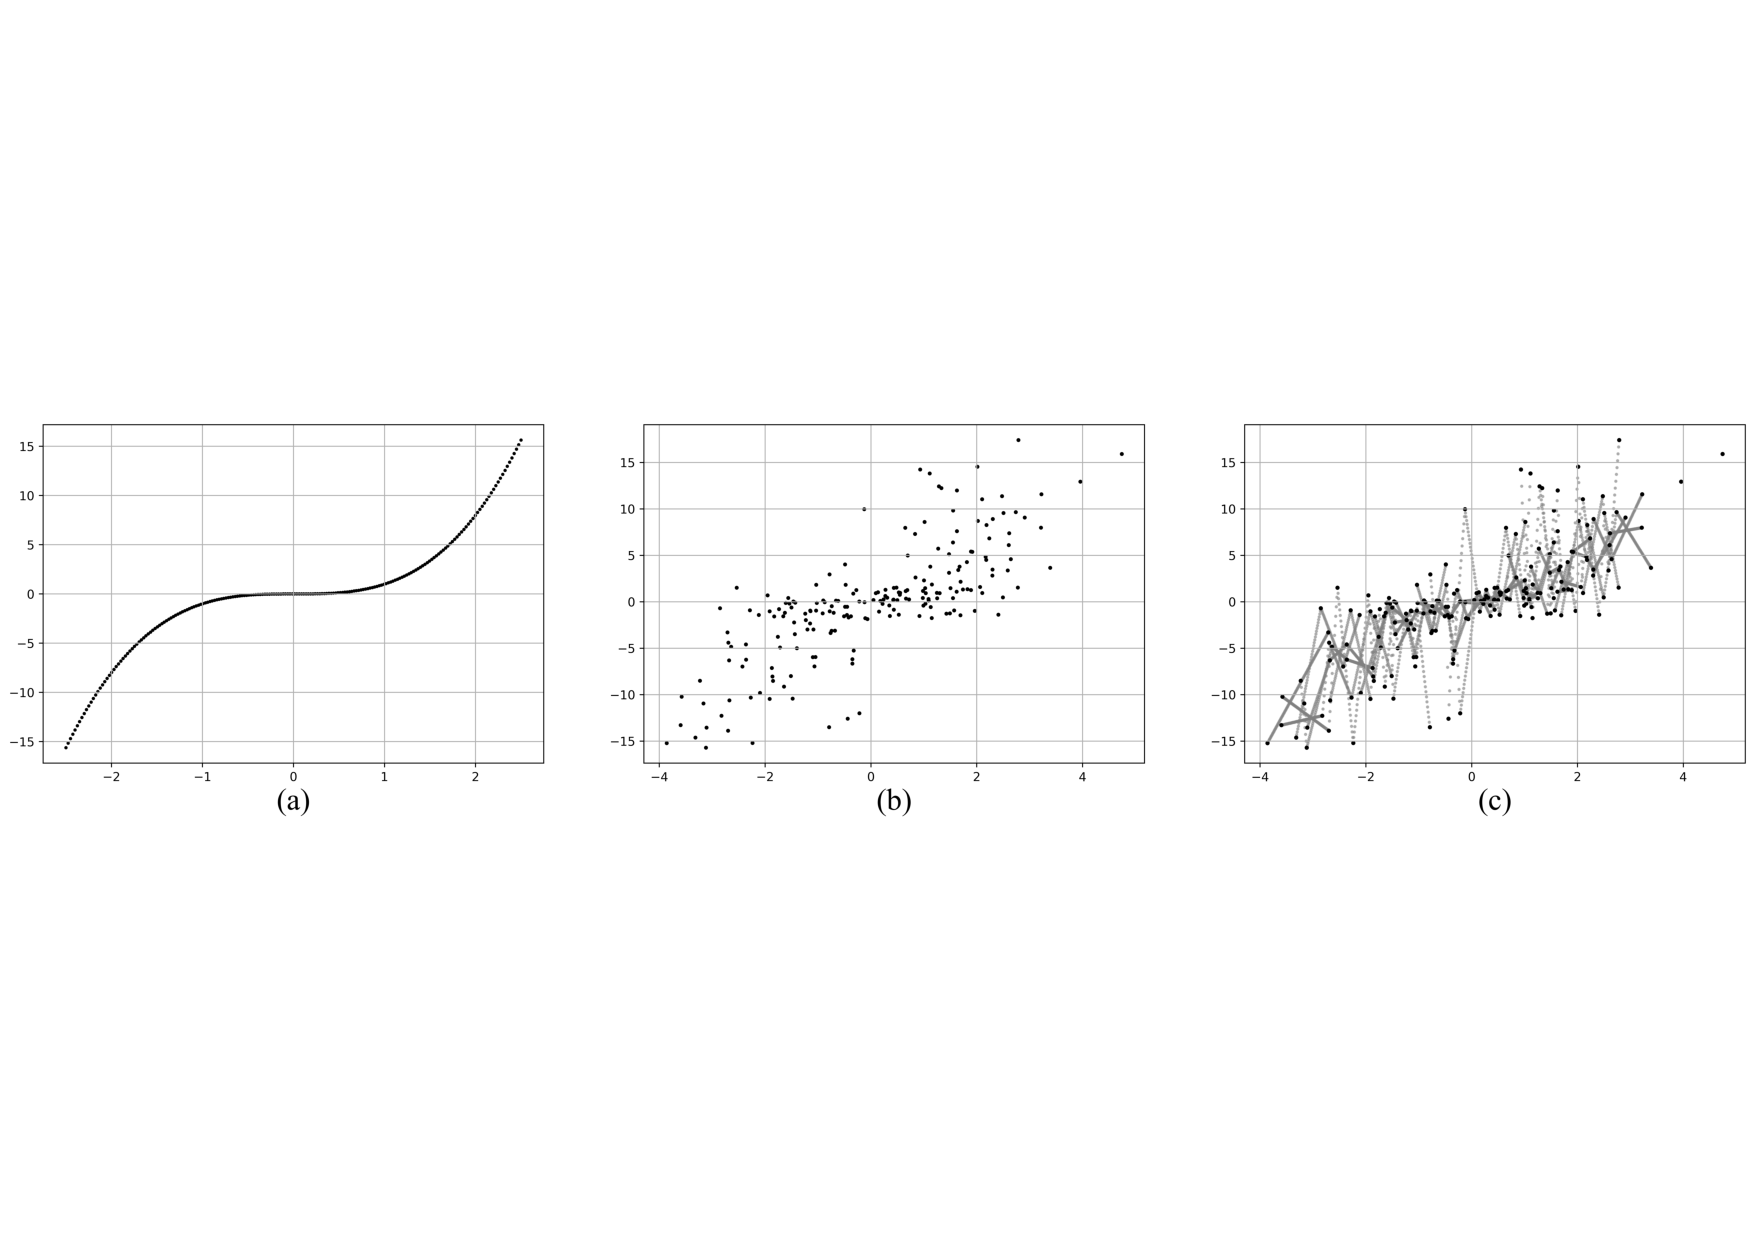
\includegraphics[width=1\textwidth]{fig2.pdf}
\caption{The synthetic data by ASISO. (a) The true relationship between $x$ and $y$, $y=x^3$. The sample size is 200. (b) Adding Gaussian noise. (c) Let $k=6,\eta=100$, processing with ASISO, the sample size was increased to 3808.}\label{fig2}
\end{figure}

The supplements about ASISO are given below:

\begin{enumerate}[2.]

\item The choice of the hyperparameter $k$ is crucial as different datasets require different values of $k$. Conversely, hyperparameter $\eta$ tends to exhibit better performance as its value increases, which will be illustrated in the following experimental results.

\item It is necessary to normalize the data if there is a significant difference in the dimensional scale between the features of the data. It avoids the issue of generating an excessive number of samples.

\item In most cases, $n/k$ is not an integer, and for the excess samples, we usually have two solutions of handling them. The first one is to use the LOF algorithm \cite{bib26} to filter out the excess samples that will not participate in the ASISO, as it is shown in Figure~\ref{fig2}(c). Another solution is to treat the excess samples as a dataset $\mathcal{D}^\prime$ of a subspace, $\mathcal{D}^\prime=\{(\boldsymbol{x}_i,y_i)\}_{{i=1}}^{{n\;mod\;k}}$.When interpolating between $\mathcal{D}^\prime$ and other subspaces $\mathcal{D}^{\prime\prime}$, choose an appropriate linear regression method to fit the dataset $\mathcal{D}^\prime\cup\mathcal{D}^{\prime\prime}$, and obtain $\hat{g}(\cdot)$. Then, use the same method to sort $\mathcal{D}^\prime$ and $\mathcal{D}^{\prime\prime}$. Only $n\;mod\;k$ interpolations are performed, with each sample in $\mathcal{D}^\prime$ being interpolated, while for $\mathcal{D}^{\prime\prime}$, only $n\;mod\;k$ samples are interpolated. Moreover, interpolate the samples with opposite signs of $\epsilon_i$ as much as possible, as it is shown in Figure~\ref{fig3}.

\end{enumerate}

\begin{figure}[H]%
\centering
\vspace{-3.9cm}   %调整图片与上文的垂直距离 
\setlength{\abovecaptionskip}{0.cm} %调整标题上方的距离 
\setlength{\abovecaptionskip}{-3.4cm} %调整标题下方的距离
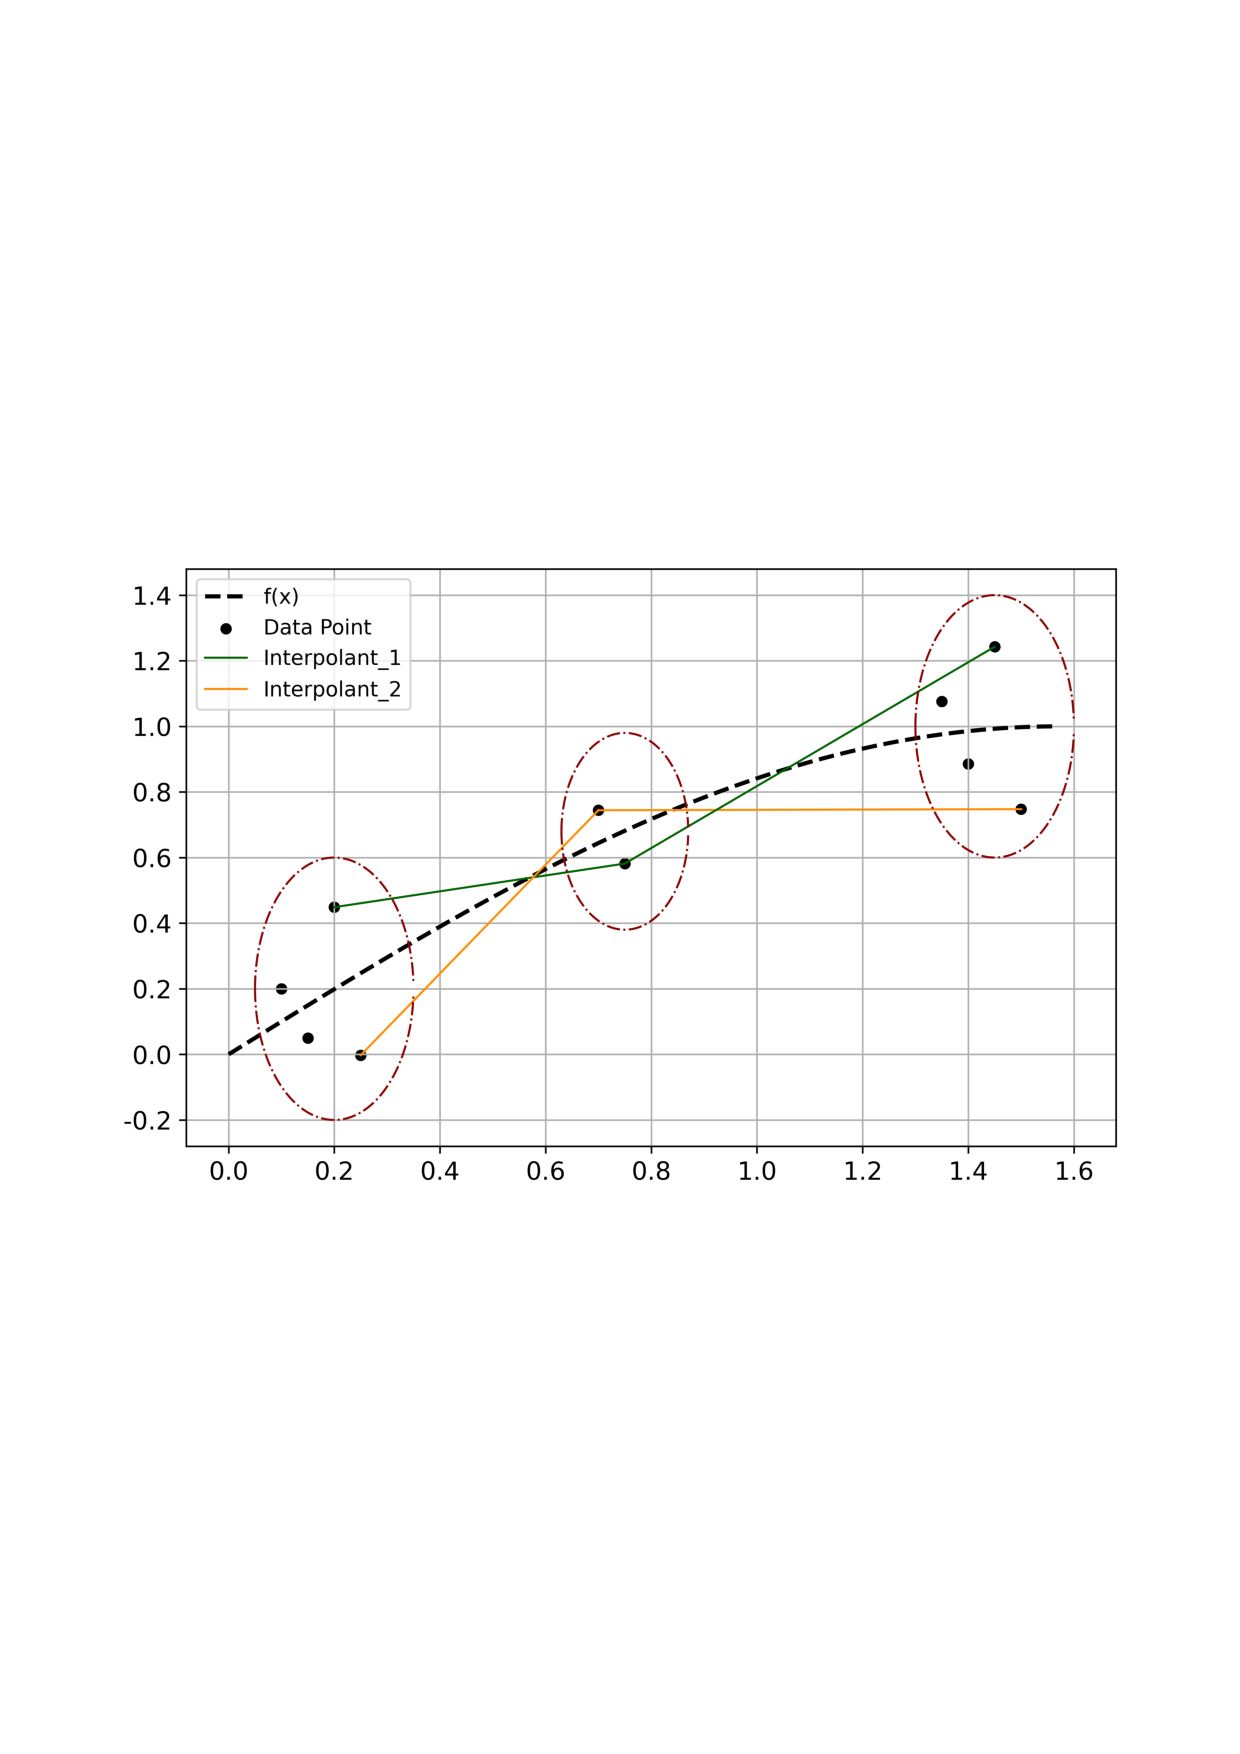
\includegraphics[width=0.6\textwidth]{fig3.pdf}
\caption{Interpolations in subspaces with different number of samples.}\label{fig3}
\end{figure}

\section{Experiments}\label{sec4}

For Artificial data, as $f(\cdot)$ can be known, we investigated the hyperparameter selection, and optimization performance after processing by ASISO. For benchmark data, we studied the prediction performance using this method.

\subsection{Artificial Data Sets}\label{subsec1}

Some verification indicators, the proportion of samples with $\epsilon_i$ greater than $\alpha$, and the mean square error (MSE), can be selected to test the optimization effect of the ASISO on the original sample after processing, as follows:

\begin{equation}
p(\alpha)=\dfrac{1}{n}\sum\limits_{i=1}^nI(|f(\boldsymbol{x}_i)-y_i|>\alpha),\label{eq13}
\end{equation}

\begin{equation}
MSE=\dfrac{1}{n}\sum\limits_{i=1}^n(f(\boldsymbol{x}_i)-y_i)^2. \label{eq14}
\end{equation}

For artificial data sets, $\{\boldsymbol{x}_i\}_{i=1}^n$ are generated by $N_p(\boldsymbol{0},\boldsymbol{E})$. Let $\boldsymbol{W}_1\in \mathbb{R}_{(p\times p_1)}$ and $\boldsymbol{W}_2\in \mathbb{R}_{(p_1\times1)}$, where all elements of both $\boldsymbol{W}_1$ and $\boldsymbol{W}_2$ are independently and identically distributed as $N(0,1)$. Consider $y_i=f(\boldsymbol{x}_i)+\epsilon_i=tanh(\boldsymbol{x}^\prime_i\boldsymbol{W}_1)\boldsymbol{W}_2+\epsilon_i$.

\begin{equation}
tanh(x)=\dfrac{e^x-e^{-x}}{e^x+e^{-x}}.\nonumber
\end{equation}

For a given data set, we typically cannot ascertain the distribution of noise. Hence, we construct datasets that contain unknown noises \cite{bib12}. The unknown noises are simulated by mixture noises that contain uniform noises and Gaussian noises. The generation of $\epsilon_i$ referenced to \cite{bib27}. We have fixed the random effects of the generated datasets; experiments are repeated 100 times in each artificial dataset. Table~\ref{tab1} shows 6 artificial datasets.

\newpage

\begin{table}[h]
\caption{Artificial Data Sets}\label{tab1}
\begin{tabular}{@{}llll@{}}
\toprule 
Artificial Data Sets & $\epsilon_i$ Distribution                                                            & Samples & $(P,P_1$) \\ \midrule
$D_1$ & \begin{tabular}[c]{@{}l@{}}20\%-N(0,64)\\ 30\%-U(-8,8)\\ 50\%-N(0,0.04)\end{tabular} & 500     & (5,3)    \\
$D_2$ & \begin{tabular}[c]{@{}l@{}}20\%-N(0,64)\\ 30\%-U(-8,8)\\ 50\%-N(0,0.04)\end{tabular} & 200     & (5,3)    \\
$D_3$ & \begin{tabular}[c]{@{}l@{}}20\%-N(0,64)\\ 30\%-U(-8,8)\\ 50\%-N(0,0.04)\end{tabular} & 1500    & (5,3)    \\
$D_4$ & \begin{tabular}[c]{@{}l@{}}20\%-N(0,64)\\ 30\%-U(-8,8)\\ 50\%-N(0,0.04)\end{tabular} & 500     & (1,3)    \\
$D_5$ & \begin{tabular}[c]{@{}l@{}}20\%-N(0,64)\\ 30\%-U(-8,8)\\ 50\%-N(0,0.04)\end{tabular} & 500     & (20,10)  \\
$D_6$ & \begin{tabular}[c]{@{}l@{}}40\%-N(0,64)\\ 45\%-U(-8,8)\\ 15\%-N(0,0.04)\end{tabular} & 500     & (5,3) \\
\botrule
\end{tabular}
\end{table}

\subsubsection{Hyperparameter Selection}\label{subsubsec1}

First, we investigate the selection of parameter $k$. To ensure that the number of feature subspaces is sufficient. We set the hyperparameter $\eta=1$, let $k=1,2,\ldots,\lfloor{\frac{n}{2}}\rfloor$. Calculate the changes in MSE of the datasets at different values of $k$, obtain $k^\prime=\mathop{argmin}\limits_{k:k=1,2,\ldots,\lfloor\frac{n}{2}\rfloor,\eta=1}MSE$. The change trend of the MSE index before and after the ASISO processing is shown in Figure~\ref{fig4}. Then, let $\eta=1,2,\ldots,30,k=k'$, calculate the changes in MSE of the datasets (Figure~\ref{fig5}), obtain $\eta^\prime=\mathop{argmin}\limits_{\eta:\eta=1,2,\ldots,30,k=k^\prime}MSE$. At last, let $k=k^\prime,\eta=1$ and $\eta^\prime$, calculate the changes in $p(\alpha)$ of the artificial datasets (Figure~\ref{fig6}).



\begin{figure}[H]%
\centering
\vspace{-0.5cm}   %调整图片与上文的垂直距离 
\setlength{\abovecaptionskip}{0.cm} %调整标题上方的距离 
\setlength{\abovecaptionskip}{-0.2cm} %调整标题下方的距离
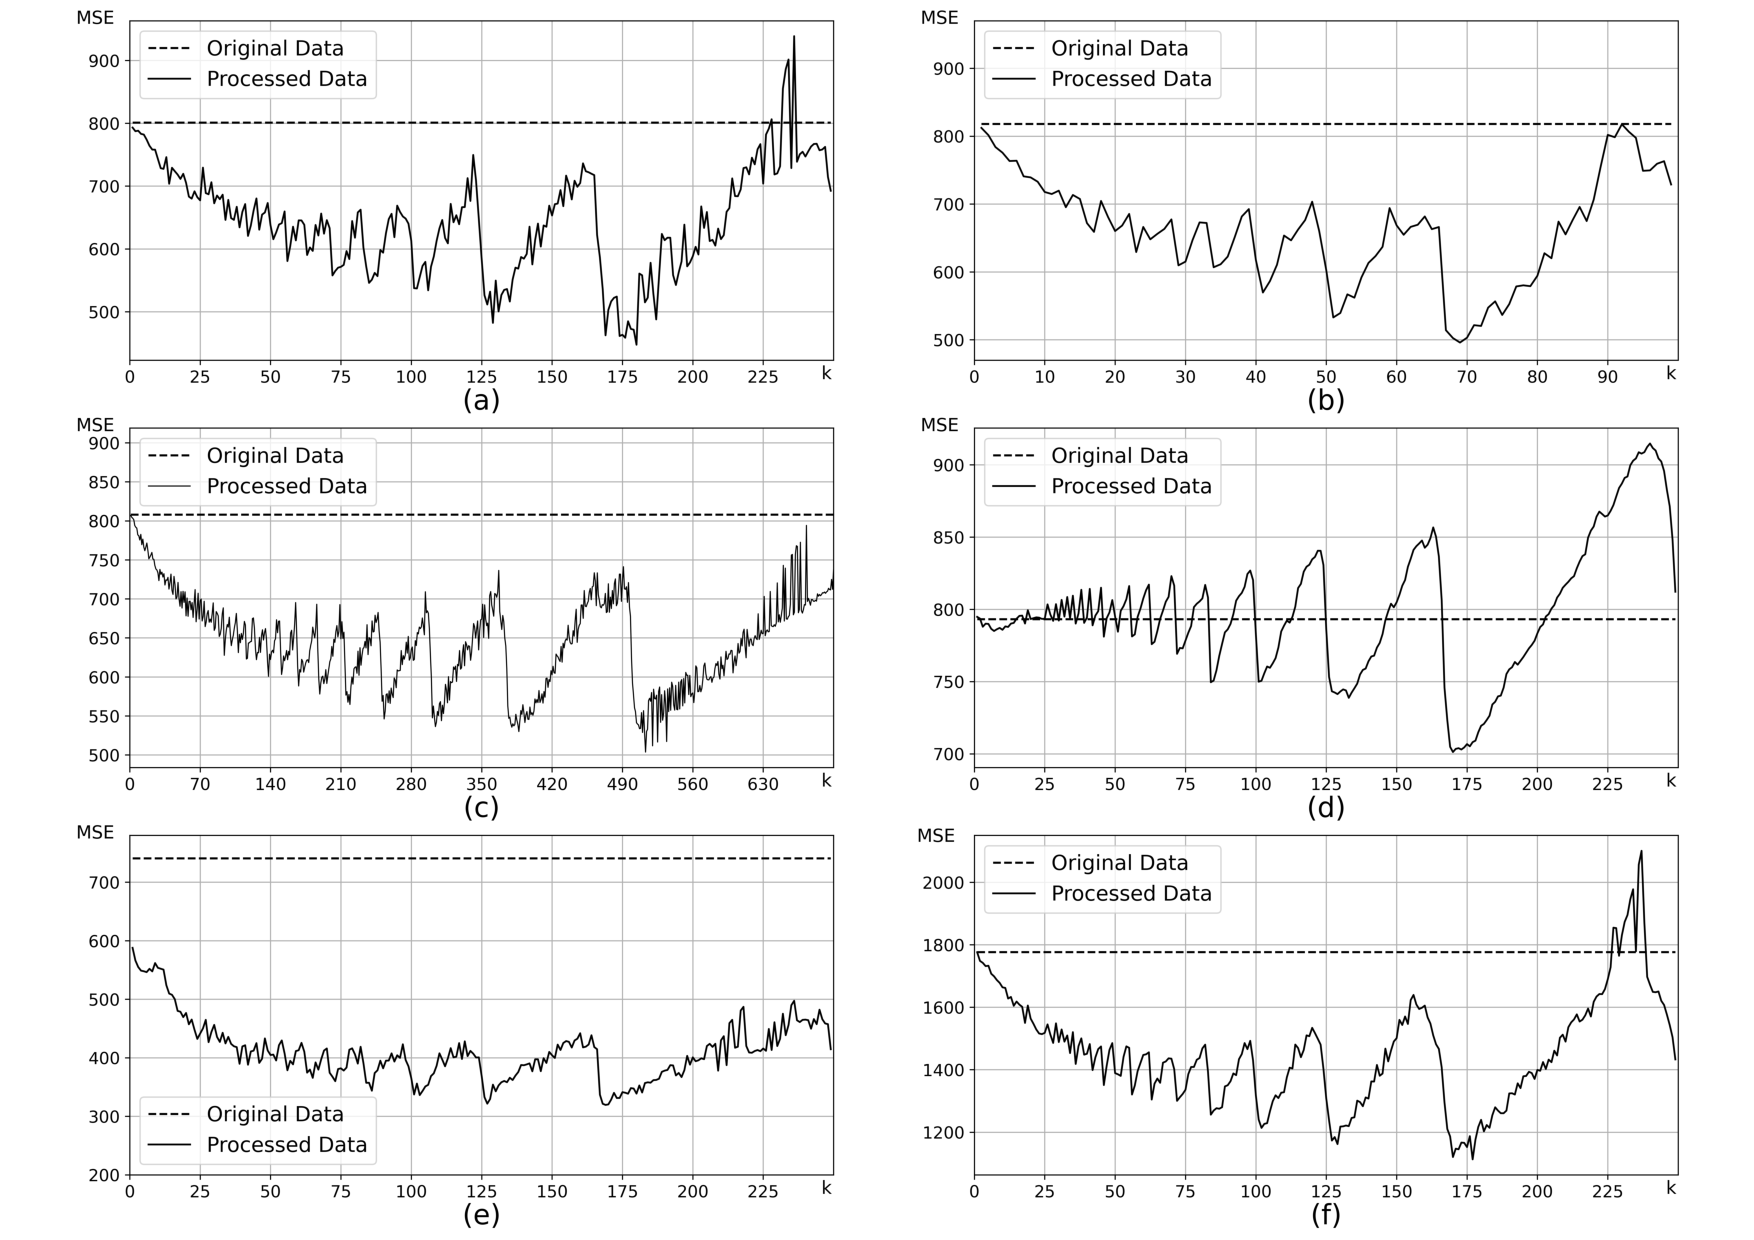
\includegraphics[width=1\textwidth]{fig4.pdf}
\caption{Changes in the MSE under different $k$ values.}\label{fig4}
\end{figure}

\begin{figure}[H]%
\centering
\vspace{-1.0cm}   %调整图片与上文的垂直距离 
\setlength{\abovecaptionskip}{0.cm} %调整标题上方的距离 
\setlength{\abovecaptionskip}{-0.2cm} %调整标题下方的距离
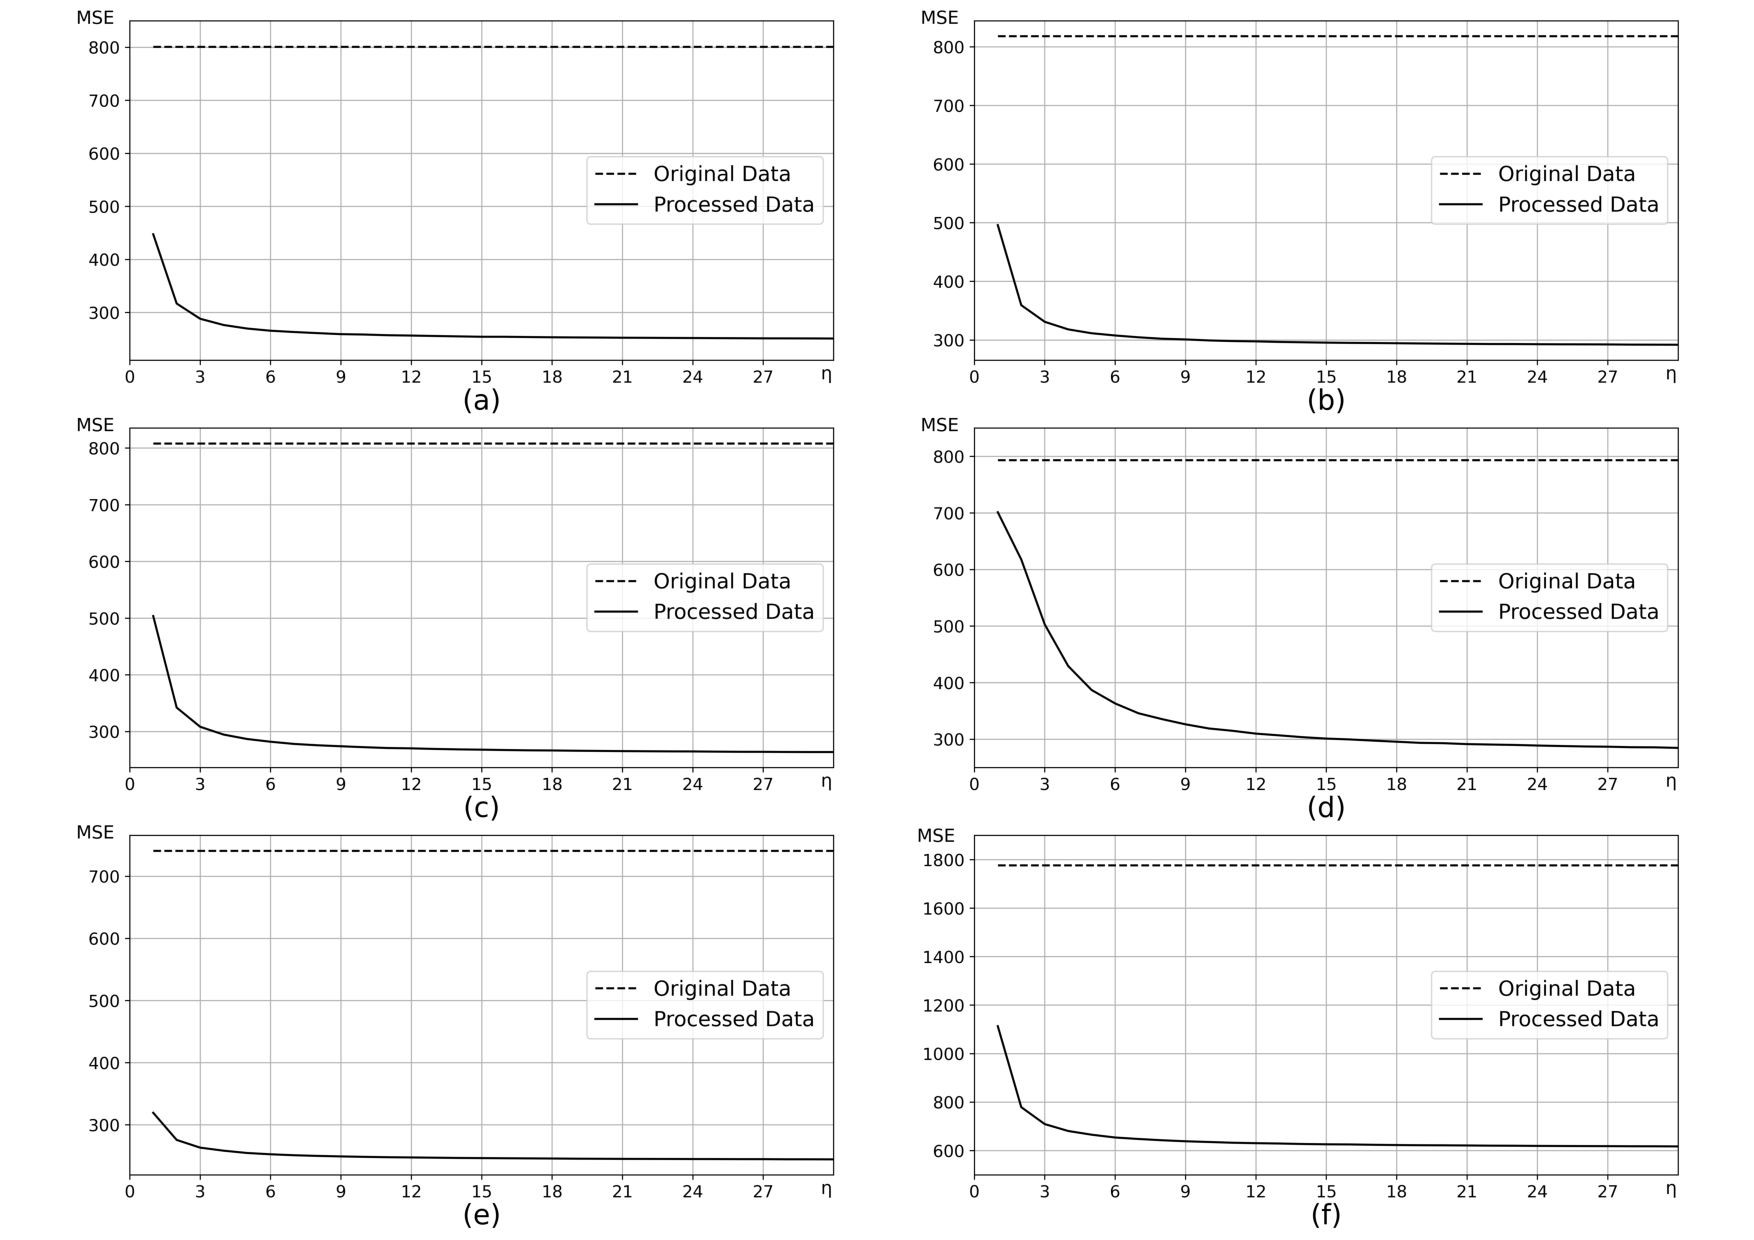
\includegraphics[width=1\textwidth]{fig5.pdf}
\caption{Changes in the MSE under different $\eta$ values.}\label{fig5}
\end{figure}

\begin{figure}[H]%
\centering
\vspace{-1.0cm}   %调整图片与上文的垂直距离 
\setlength{\abovecaptionskip}{0.cm} %调整标题上方的距离 
\setlength{\abovecaptionskip}{-0.2cm} %调整标题下方的距离
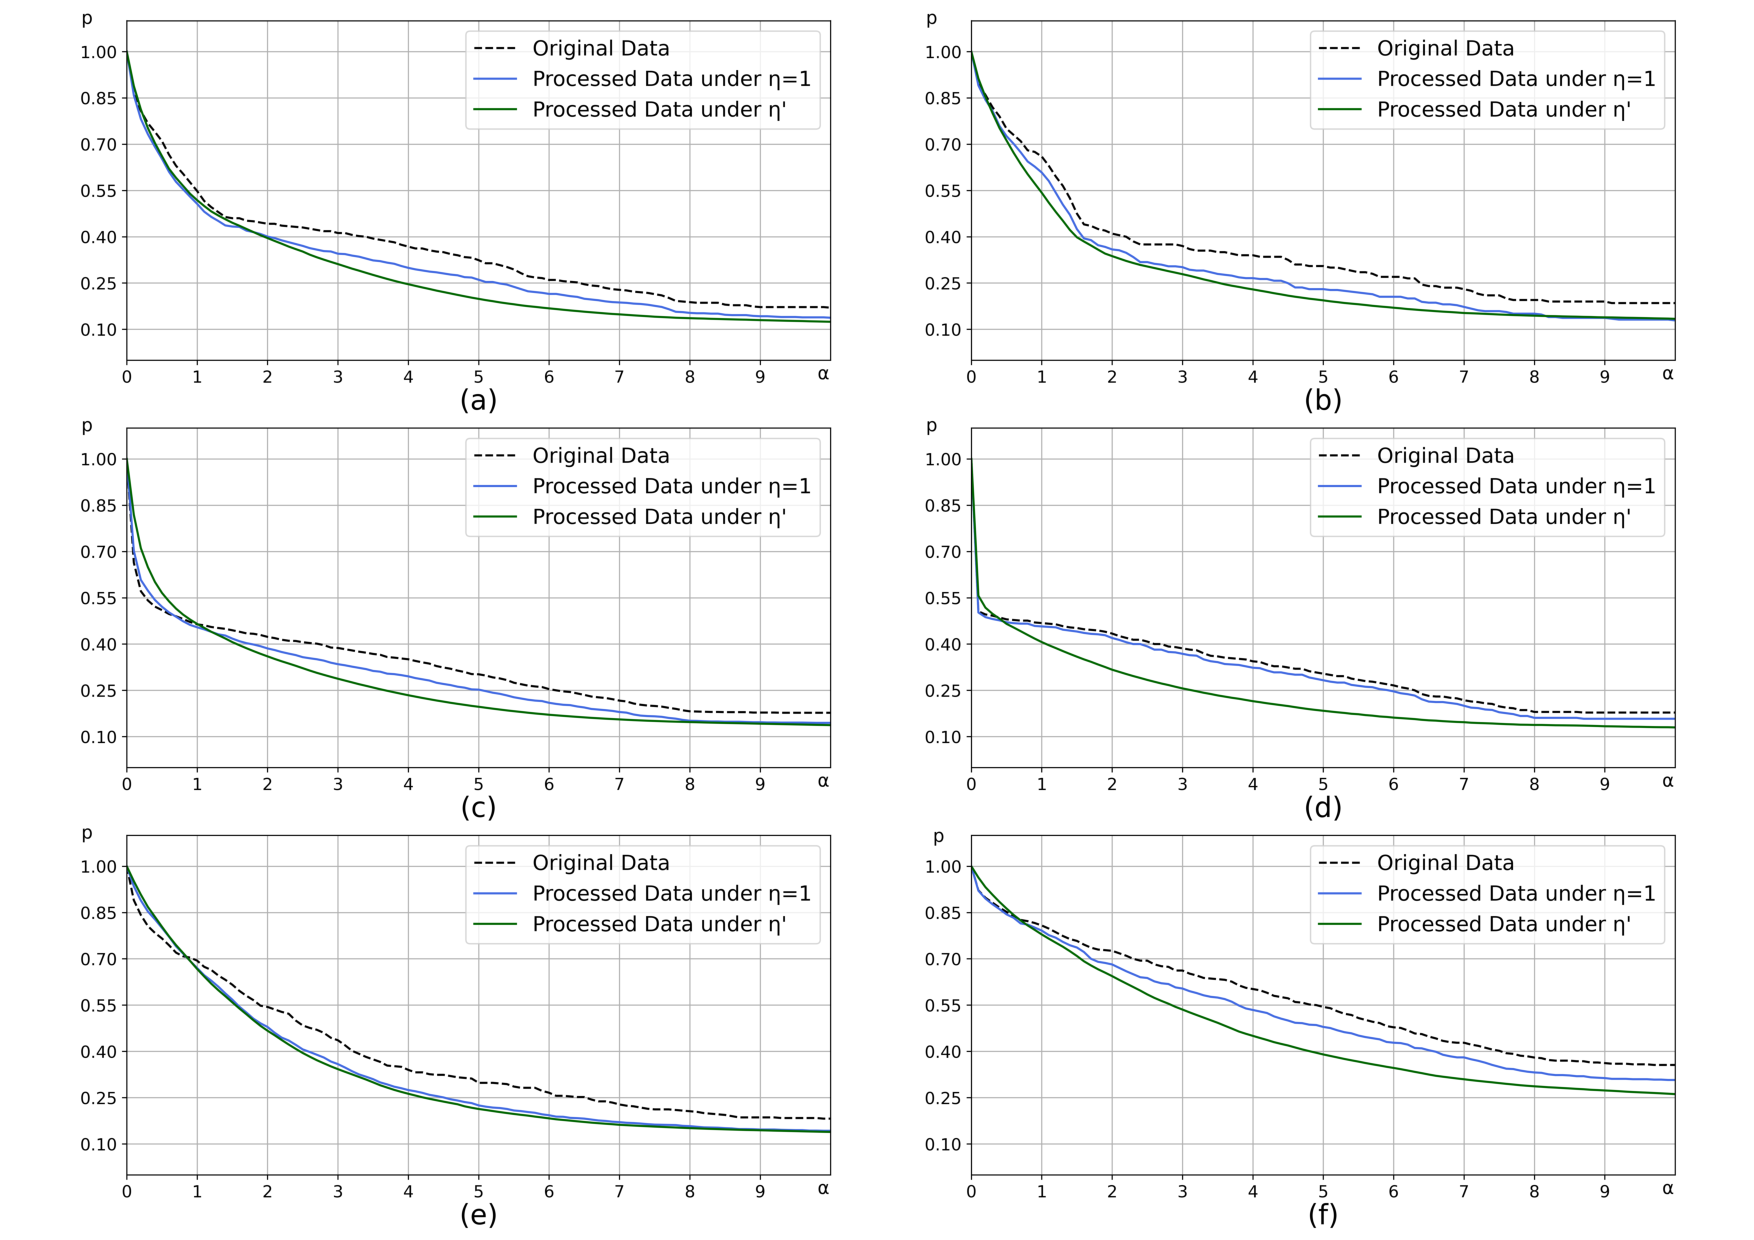
\includegraphics[width=1\textwidth]{fig6.pdf}
\caption{Changes in the $p(\alpha)$ under different $\eta$ values.}\label{fig6}
\end{figure}

As can be seen from Figure~\ref{fig4}, ASISO demonstrates good optimization performance for datasets with varying sample sizes or feature dimensions. Experimental results also show that the performance of ASISO does not decline dramatically as the content of noise with large variances increases. Hence, it can deal with unknown noise better and has good robustness. In addition, it can be shown that ASISO exhibits good optimization performance for all datasets from experimental results, it is also a stable data synthesis method. As can be seen from Figure~\ref{fig5}, the hyperparameter $\eta$ has a generally monotonically decreasing relationship with MSE, and the larger the value of $\eta$, the more significant the effect. From Figure~\ref{fig6}, it can be observed that ASISO can adaptively adjust the sample structure, which reduces the proportion of samples with large errors.

\subsubsection{Comparison of Optimization Performance}\label{subsubsec2}

To verify the optimization performance of ASISO, it is compared three methods: piecewise linear interpolation, linear extrapolation, and nearest neighbor interpolation. Specifically, let $k=k^\prime,\eta=\eta^\prime$ in ASISO. Based on the given dataset, we use the samples generated by ASISO as interpolation points to calculate the output values in linear extrapolation and nearest neighbor interpolation. Moreover, let $k=1$ and $\eta=\eta^\prime$ in ASISO, we can regard it as piecewise linear interpolation. The experimental results show that ASISO has the smallest MSE among all methods for each dataset (Figure~\ref{fig7}). 

\begin{figure}[H]%
\centering
\vspace{-1.0cm}   %调整图片与上文的垂直距离 
\setlength{\abovecaptionskip}{0.cm} %调整标题上方的距离 
\setlength{\abovecaptionskip}{-1.4cm} %调整标题下方的距离
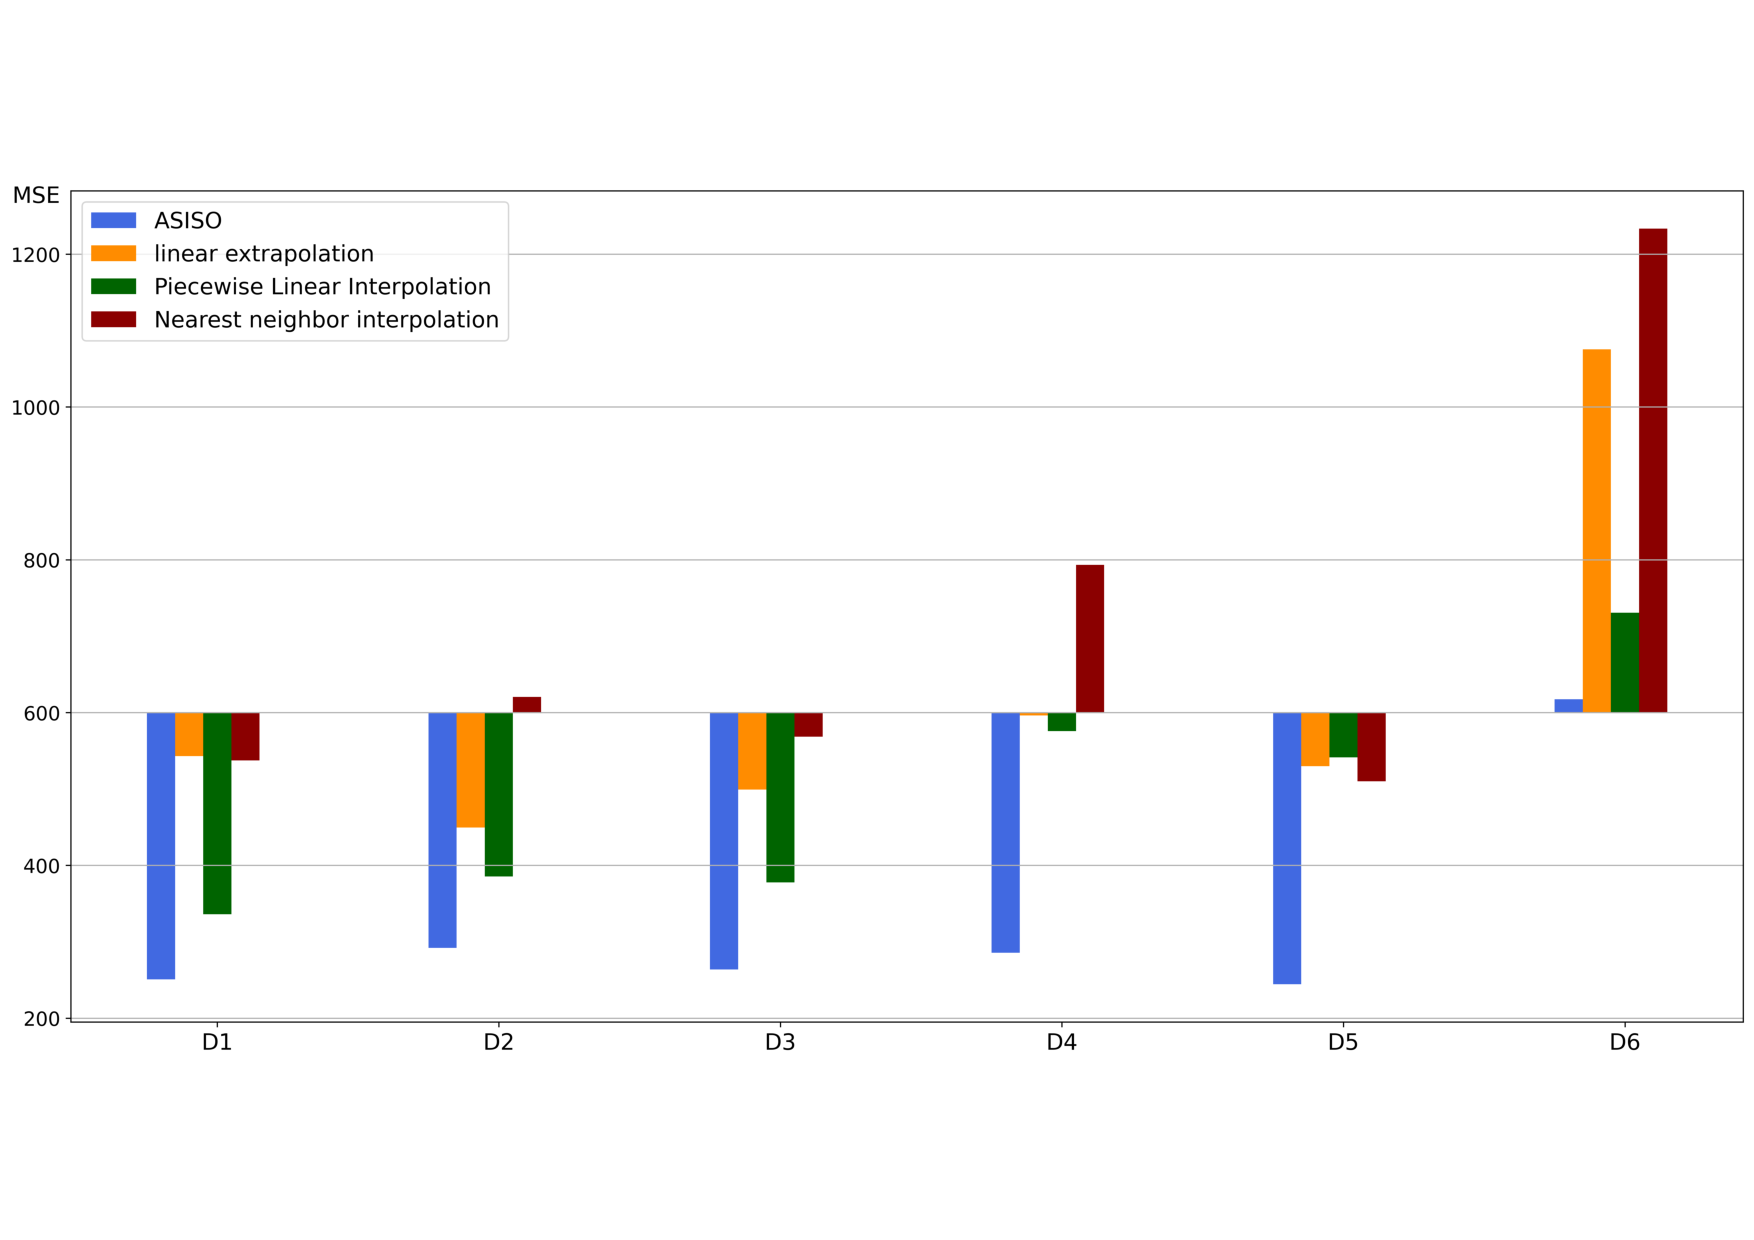
\includegraphics[width=1\textwidth]{fig7.pdf}
\caption{Comparison of MSE on artificial data sets.}\label{fig7}
\end{figure}

\begin{sidewaystable}[]
\caption{Experimental Results on Benchmark Data Sets}\label{tab2}
\begin{tabular*}{\textheight}{@{\extracolsep\fill}lllllllll}
\toprule%
\multirow{2}{*}{Data sets}           & \multirow{2}{*}{Processing} & \multirow{2}{*}{Hyperparameter} & \multirow{2}{*}{Training set size} & \multicolumn{5}{c}{Testing set MAE($10^-2$)}                                                                      \\ \cmidrule{5-9}
                                     &                             &                                 &                                    & KNN                & RF                 & MLP                 & SVR                 & GBDT               \\ \hline
\multirow{2}{*}{Bike Sharing Demand} & -                           & -                               & 7620                               & $2.20$  & $\boldsymbol{0.12}$ & $0.54$   & $4.26$ & $0.23$ \\
                                     & ASISO                       & $k=150,\eta=10$                 & 40380                              & $2.00$    & $\boldsymbol{0.06}$    & $0.25$   & $4.12$  & $0.19$  \\
\multirow{2}{*}{Facebook Metrics}    & -                           & -                               & 346                                & $6.60$  & $2.25$ & $8.19$  & $7.34$  & $\boldsymbol{1.33}$ \\
                                     & ASISO                       & $k=2,\eta=10$                   & 1450                               & $6.41$ & $1.59$ & $2.02$  & $7.36$  & $\boldsymbol{1.12}$ \\
\multirow{2}{*}{Air Quality}         & -                           & -                               & 6549                               & $2.99$ & $\boldsymbol{2.57}$ & $4.80$   & $3.87$  & $2.58$ \\
                                     & ASISO                       & $k=20,\eta=100$                 & 101984                             & $2.89$ & $2.55$ & $\boldsymbol{2.08}$  & $3.84$  & $2.77$ \\
\multirow{2}{*}{Forest Fires}        & -                           & -                               & 361                                & $\boldsymbol{4.06}$ & $4.93$ & $10.58$ & $7.36$  & $4.49$ \\
                                     & ASISO                       & $k=10,\eta=100$                 & 21131                              & $\boldsymbol{3.89}$ & $4.32$ & $4.80$   & $10.05$ & $4.14$ \\
\botrule
\end{tabular*}
\end{sidewaystable}


\subsection{Benchmark Data Sets}\label{subsec2}

To verify the prediction performance of ASISO, 4 benchmark data sets are used \cite{bib28,bib29}. We partitioned the dataset into training and testing sets using a 7:3 ratio and normalize the data using the min-max normalization method. We preprocessed the training data using ASISO, train multiple machine learning models on the training set, and evaluated the prediction performance of the models on the testing set. The evaluation metric we used was mean absolute error (MAE). 

\begin{equation}
MAE=\dfrac{1}{n}\sum\limits_{i=1}^n|y_i-\hat{y}_i|.\label{eq15}
\end{equation}

In addition, we removed features that cannot be directly used, such as "Datetime" for bike sharing demand, "Month" for forest fires, and so on. We choose K-Nearest Neighbor (KNN), Random Forest (RF), Gradient Boosting Decision Tree (GBDT), Multilayer Perceptron (MLP) and Support Vector Regression (SVR) as the machine learning prediction models. Specifically, the kernel function is Radial Basis Function (RBF) in SVR. Moreover, set the number of hidden layers to 3 for the MLP and use different numbers of neurons based on the input dimensionality and sample size. 

The experimental results of the five models are shown in Table~\ref{tab2}. It is evident that ASISO performs well on each benchmark dataset. This method is highly applicable to all five models, and in most cases, it can improve the predictive performance. It is worth mentioning that the dataset contains many categorical features, which are not continuous variables. Moreover, for sparse samples (Facebook Metrics and Forest Fires), it is difficult to guarantee that the linear fitting error $\epsilon^\prime_i\rightarrow0$ when interpolating between subspaces. This indicates that even if there are violations of the ASISO assumptions in practical applications, this method may still achieve good optimization results. This further demonstrates that it is robust and stable.


\section{Conclusion}\label{sec5}

In this paper, we propose a data synthesis method, ASISO, which can adaptively adjust the size of the dataset, and the expanded data typically contain minimal error with actual. Moreover, it can adjust the structure of the samples, which can significantly reduce the proportion of samples with large errors. The experimental results on artificial data sets demonstrate that ASISO can optimize the samples, and compared to other methods, the generated data using this method has smaller errors. It can deal with unknown noise better and has good robustness. The results on benchmark data sets show the proposed method is applicable to many machine models, and in most cases, it can improve the model generalization.

%----------------------------------------------------------------------%


\bibliography{sn-bibliography}% common bib file
%% if required, the content of .bbl file can be included here once bbl is generated
%%\input sn-article.bbl


\end{document}
